\documentclass[a4paper]{article}

%% Language and font encodings
\usepackage[english]{babel}
\usepackage[utf8x]{inputenc}
\usepackage[T1]{fontenc}
\usepackage{tikz}
\usetikzlibrary{arrows,automata, backgrounds, fit}

%% Sets page size and margins
\usepackage[a4paper,top=3cm,bottom=2cm,left=3cm,right=3cm,marginparwidth=1.75cm]{geometry}

%% Useful packages
\usepackage{amsmath}
\usepackage{graphicx}
\usepackage[colorinlistoftodos]{todonotes}
\usepackage[colorlinks=true, allcolors=blue]{hyperref}

\begin{document}

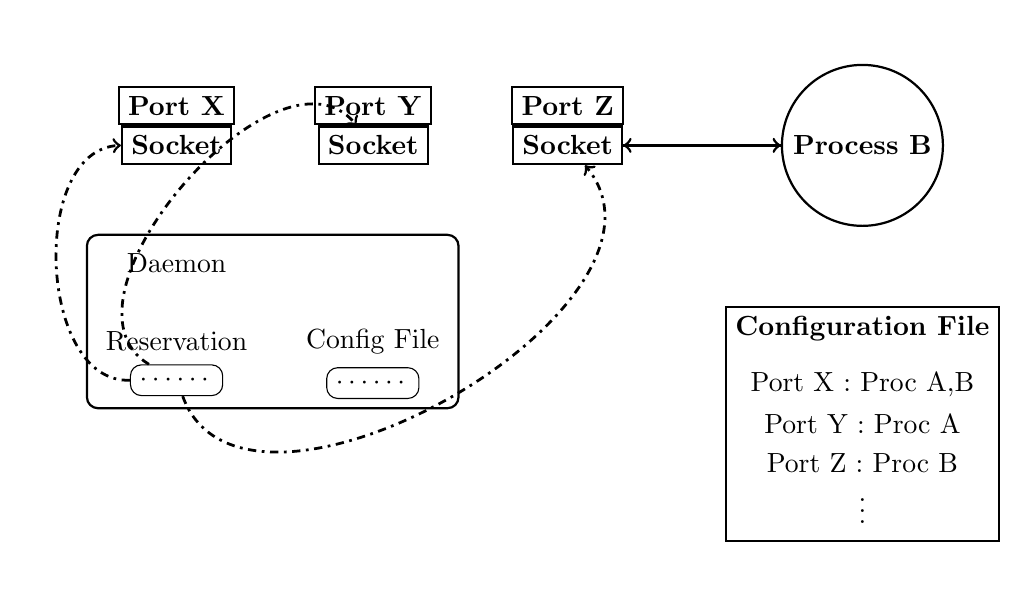
\begin{tikzpicture}
	\node(portX) [draw, thick]{\textbf{Port X}};
    \node(portY) [draw, thick, right=of portX]{\textbf{Port Y}};
    \node(portZ) [draw, thick, right=of portY]{\textbf{Port Z}};
    
    \node(sockX) [draw, thick, below=0cm of portX]{\textbf{Socket}};
    \node(sockY) [draw, thick, below=0cm of portY]{\textbf{Socket}};
    \node(sockZ) [draw, thick, below=0cm of portZ]{\textbf{Socket}};
    
    \node(procB) [draw, thick, circle, right=2cm of sockZ]{\textbf{Process B}};
    \draw[->, line width=1pt] (sockZ) edge (procB) (procB) edge (sockZ);
    
    %\node(daemon) [draw, thick, below=2cm, text depth=3cm, minimum width=7cm, minimum height=3cm]{\textbf{\Large Daemon}};
    
    \tikzstyle{bigbox} = [draw, thick, rounded corners, rectangle]
	\tikzstyle{box} = [rounded corners,rectangle]
	\node[box, below=of sockX] (daemon) {Daemon};
	\node[box, below=0.5cm of daemon] (res) {Reservation};
	\node[box, right=0.5cm of res] (conf) {Config File};
	\node[box, below=0.05cm of res, draw, rectangle] (res_box) {$\cdots \cdots$};
	\node[box, below=0.05cm of conf, draw, rectangle] (conf_box) {$\cdots \cdots$};

	\begin{pgfonlayer}{background}
  		\node[bigbox] [fit = (daemon) (conf) (res) (res_box) (conf_box)] {};
	\end{pgfonlayer}
	
	\path
		(res_box) edge[->, bend left=90, line width=1pt, dash dot] node [] {} (sockX)
		(res_box) edge[->, bend left=100, line width=1pt, dash dot] node [] {} (sockY)
		(res_box) edge[->, bend right=100, line width=1pt, dash dot] node [] {} (sockZ);

	\node(conf) [draw, thick, below=1cm, text depth=2.5cm, minimum width=3cm, below=1cm of procB]{\textbf{Configuration File}};
    \node at ([yshift=-1cm]conf.north){Port X : Proc A,B};
    \node at ([yshift=-1.5cm]conf.north){Port Y : Proc A};
    \node at ([yshift=-2cm]conf.north){Port Z : Proc B};
    \node at ([yshift=-2.5cm, sloped]conf.north){$\vdots$};
\end{tikzpicture}

\end{document}